\documentclass[11pt,journal,onecolumn]{IEEEtran}
\usepackage[margin=1in]{geometry}
\usepackage{amsmath,amssymb}
\usepackage{graphicx}
\usepackage{booktabs}
\usepackage{array}
\usepackage{cite}
\usepackage{url}
\usepackage{xcolor}
\usepackage{tikz}
\usetikzlibrary{positioning,arrows.meta}
\usepackage[hidelinks]{hyperref}
\usepackage{microtype}

\begin{document}

\title{Matching Food Descriptions to FNDDS Codes with Hybrid Retrieval and a Probabilistic Decision Model}
\author{Brayden~Abo}
\markboth{DRAFT}{ABO: MATCHING FOOD DESCRIPTIONS TO FNDDS CODES WITH HYBRID RETRIEVAL AND A DECISION MODEL}
\maketitle

\begin{center}\begin{minipage}{0.92\linewidth}\small\noindent
{\bfseries\itshape Abstract}{\bfseries ---Turning a dietary log into nutrient estimates requires mapping each free-text food description to an entry in a food composition database, a step that is still often done by hand. Automating it is difficult for three reasons. The USDA Food and Nutrient Database for Dietary Studies (FNDDS) contains 5,432 foods, more than a single query to a language model can consider. Many foods differ only in preparation or form. Real inputs contain brand names, typos, and missing details. We introduce a two-stage matcher that shortlists candidates with four complementary retrievers merged by reciprocal-rank fusion, and then asks Jev, a hosted decision model that returns a probability for every option, to choose a code or abstain. We evaluated the matcher on 279 hand-labeled foods. The shortlist contained the correct code for 89.6\% of foods, and Jev increased exact-code top-1 accuracy from 44.1\% (retrieval alone) to 59.1\%. When a wrong code with nearly identical per-100\,g macronutrients was counted as acceptable, accuracy was 78.1\%. Jev's probabilities were overconfident (expected calibration error 0.22), but a confidence threshold of 0.96 fitted on half of the foods accepted 40.9\% of the other half at 92.9\% precision. Errors came mainly from underspecified inputs and near-duplicate codes, not from mistakes across food categories, and evaluating all 279 foods cost about one cent. Many foods can therefore be matched automatically at low cost while uncertain cases are routed to review.}

\medskip\noindent
{\bfseries\itshape Index Terms}---Dietary assessment, food composition database, FNDDS, information retrieval, large language models, calibration.
\end{minipage}\end{center}

\section{Introduction}
\IEEEPARstart{U}{nderstanding} what people eat requires more than a list of foods. To estimate energy and nutrient intake, each reported food must be linked to an entry in a food composition database. In the United States, the Food and Nutrient Database for Dietary Studies (FNDDS) serves this role for national dietary surveys, assigning each of its foods a code with per-100\,g nutrient values~\cite{fndds}. The linking step is labor intensive when done by hand; one effort to map dairy foods to a composition database was reported to take about 28 minutes per food~\cite{lemay}. Automated matching would make it practical to code large dietary datasets, to support food logging applications, and to harmonize records across databases that change over time.

Automated matching is difficult for three reasons. First, the database is large: FNDDS has 5,432 foods, and a single multiple-choice question to a model can hold at most a few hundred options. Second, specificity matters. ``Carrots'' can mean raw, boiled, or fried-with-fat carrots, each a different code with different nutrients, and the same food appears at many levels of detail. Third, inputs are noisy, containing brands (``Talenti sorbet''), typos (``Crakers''), abbreviations (``PB''), and descriptions that omit how the food was prepared. Approaches based on string similarity, term frequency, or text embeddings retrieve plausible candidates but cannot reliably pick among near-duplicates, while language models given an entire database perform poorly and can return foods that are not in it~\cite{lemay}. The most accurate published approach combines the two: embeddings select a short list, and a language model chooses among the candidates or answers ``No Match''~\cite{lemay}.

We build on this two-stage design and ask whether it can be made more usable in practice. Two features of practical use motivate our changes. A system that knows when it is uncertain can accept confident matches automatically and send the rest to a person, which requires a confidence signal that can be trusted. And when matches feed nutrient calculations, a wrong code whose nutrients are almost identical to the correct one is a cheap error, so exact-code accuracy alone understates usefulness. We therefore combine four complementary retrievers instead of one, use a decision model that returns a probability for every option~\cite{jev}, and evaluate not only accuracy but calibration, selective acceptance, and nutrient closeness.

Our key contributions are as follows:
\begin{itemize}
\item A retrieve-then-choose matcher for FNDDS that fuses fuzzy, character n-gram, head-noun, and embedding retrieval, with a measured ablation of each combination.
\item An evaluation on 279 hand-labeled foods that includes a retrieval-only baseline, a fit/test split for threshold selection, and a nutrient-aware correctness measure. Jev improved exact-code top-1 accuracy from 44.1\% to 59.1\%, and accuracy was 78.1\% when nutritionally equivalent codes were accepted.
\item A finding that the model's confidence is overconfident (expected calibration error 0.22) yet can be thresholded: at a confidence of 0.96 or higher, held-out precision was 92.9\% while accepting 40.9\% of foods.
\item An error analysis showing that mistakes come mainly from underspecified inputs and near-duplicate codes, and open code with a one-command data download.
\end{itemize}

\section{Related Work}
\subsection{Mapping Foods to Food Composition Databases}
Linking dietary records to composition databases has traditionally relied on manual review by trained staff, which is accurate but does not scale~\cite{lemay}. Automated methods include string similarity, term frequency--inverse document frequency (TF-IDF), and text embeddings, which rank database entries by their similarity to the input. Lemay \emph{et al.}~\cite{lemay} compared these methods with large language models on two benchmarks that map dietary descriptions to other food databases. Their best system was hybrid: an embedding model (GTE-large~\cite{gte}) selected the top candidates and a language model chose among them or answered ``No Match.'' They also reported that a similarity threshold could not separate match from no-match, that a language model given a whole database performed poorly and could return foods that were not in it, and that an explicit ``none'' option improved results. We adopt the two-stage structure and the abstain option. Our work differs in the retrieval stage (four fused retrievers rather than an embedding alone), in the decision model (one that returns a probability per option, enabling threshold fitting), in the target (FNDDS with its nutrient values), and in the inputs (short noisy strings rather than database descriptions).

\subsection{Candidate Retrieval and Rank Fusion}
Lexical retrievers match surface text and tolerate typos, while dense retrievers embed text in a vector space and match by meaning~\cite{bge,gte}. Their errors differ, which makes them good candidates for combination. Reciprocal-rank fusion (RRF) merges ranked lists by summing $1/(k+\mathrm{rank})$ for each item across lists and has been shown to outperform both individual rankers and several learned combination methods~\cite{rrf}. Because it uses only ranks, it needs no score calibration across retrievers with incompatible scales.

\subsection{Confidence and Selective Prediction}
Modern classifiers are often overconfident, meaning their stated probabilities exceed their observed accuracy~\cite{guo}. Calibration is commonly summarized by the expected calibration error (ECE)~\cite{naeini}. Selective classification lets a system abstain when its confidence is low, trading coverage for accuracy~\cite{geifman}. For dietary matching this trade-off is central: a matcher that can accept confident matches and defer the rest lowers the manual effort without lowering data quality, provided its confidence can be thresholded reliably.

\section{Methods}
We begin by describing the matching pipeline. We then describe the databases and labeled data, the experiments, and the evaluation metrics.

\subsection{Matching Pipeline}
Fig.~\ref{fig:pipeline} shows the pipeline. A food description, with optional context such as portion size or brand, is normalized, used to retrieve and fuse candidates from FNDDS, presented to Jev as a choice question, and converted to a decision.

\begin{figure*}[!tb]
\centering
\resizebox{\linewidth}{!}{%
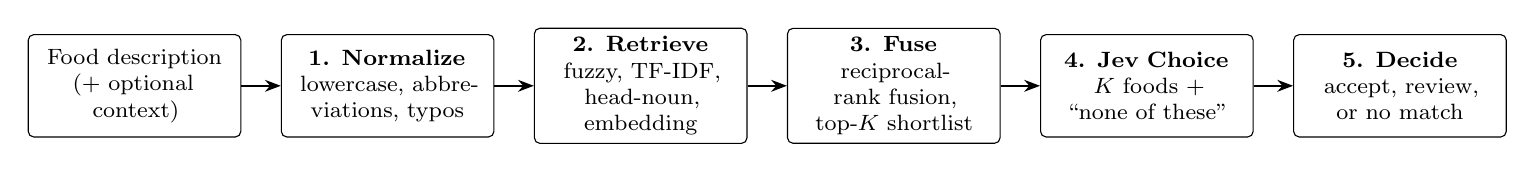
\begin{tikzpicture}[
  font=\footnotesize,
  box/.style={draw, rounded corners=2pt, align=center, text width=0.98in, minimum height=13mm, inner sep=3pt},
  arr/.style={-{Stealth[length=2mm]}, thick},
  node distance=5mm]
\node[box] (in) {Food description\\(+ optional context)};
\node[box, right=of in] (norm) {\textbf{1. Normalize}\\lowercase, abbreviations, typos};
\node[box, right=of norm] (ret) {\textbf{2. Retrieve}\\fuzzy, TF-IDF, head-noun, embedding};
\node[box, right=of ret] (fuse) {\textbf{3. Fuse}\\reciprocal-rank fusion, top-$K$ shortlist};
\node[box, right=of fuse] (jev) {\textbf{4. Jev Choice}\\$K$ foods + ``none of these''};
\node[box, right=of jev] (dec) {\textbf{5. Decide}\\accept, review, or no match};
\foreach \a/\b in {in/norm, norm/ret, ret/fuse, fuse/jev, jev/dec} \draw[arr] (\a) -- (\b);
\end{tikzpicture}}
\caption{Overview of the matching pipeline. Steps 1--3 run locally; step 4 is a single request to Jev that returns a probability for every option.}
\label{fig:pipeline}
\end{figure*}

\subsubsection{Normalization}
Descriptions are lowercased, stripped of punctuation, and cleaned with an abbreviation dictionary (e.g., ``pb'' to ``peanut butter'') and a small typo dictionary. The original string is kept alongside the normalized one.

\subsubsection{Candidate Retrieval}
Four retrievers each return a ranked list of FNDDS foods. \emph{Fuzzy} scores token-set and partial string similarity over main and additional descriptions. \emph{TF-IDF} compares character 3--5-grams, which tolerates typos and word order. \emph{Head-noun} matches the query against the text before an entry's first comma, where FNDDS places the food name, and scores
\begin{equation}
s_{\mathrm{head}}(q,e)=\frac{h}{|q|}\sqrt{\frac{h}{|H_e|}}
\end{equation}
where $h$ is the number of words shared by the query $q$ and the entry's head $H_e$, so a generic query such as ``egg'' favors ``Egg, whole, boiled'' over ``Roll, egg bread.'' \emph{Embedding} ranks foods by the cosine similarity of the query and description vectors from a small embedding model, bge-small~\cite{bge}. The four lists are merged by RRF~\cite{rrf}:
\begin{equation}
s_{\mathrm{RRF}}(e)=\sum_{r}\frac{1}{60+\mathrm{rank}_r(e)}
\end{equation}
and the top $K=30$ foods form the shortlist.

\subsubsection{Choice with Jev}
Jev is a hosted decision model that answers typed questions about a text state and returns a probability for each option~\cite{jev}. The shortlist plus a ``none of these'' option is sent as one Choice question. The question carries the food string, the optional context, and, for each option, its brand and alias text as a description. Jev returns a probability $p_j$ for every option $j$. A food is \emph{accepted} if the top option is not ``none of these'' and
\begin{equation}
p_1\ge t \quad\text{and}\quad p_1-p_2\ge m
\end{equation}
where $p_1$ and $p_2$ are the two highest probabilities and $t$ and $m$ are thresholds; otherwise it is sent to review, or reported as no match when ``none of these'' is top. Because a Choice answer can only be one of the supplied options, the model cannot return a food that is not in the shortlist. Shuffle-averaging and a yes/no verification step are implemented but not evaluated here.

\subsection{Data}
\subsubsection{FNDDS}
We used the FNDDS 2021--2023 release~\cite{fndds} distributed through FoodData Central (release 2024-10-31), which has 5,432 foods. Each has a main description, optional additional descriptions (brands and aliases), and per-100\,g energy, protein, carbohydrate, and fat. No two foods share a description, so descriptions serve as unique option strings. The first digit of an FNDDS code identifies one of nine major food groups, and the leading digits encode subgroups.

\subsubsection{Labeled Foods}
We evaluated on 279 food components from a private set of meal-photo annotations (not released), each with a hand-assigned FNDDS code. Fig.~\ref{fig:groups}(a) shows the distribution across major food groups. Only 221 distinct strings appear; 37 strings repeat, covering 95 rows, so errors on repeated foods are correlated and the effective sample is smaller than 279. Eleven labels pointed to codes absent from the 2021--2023 release, and we remapped them by judgment to the closest current code; about nine more appear wrong or ambiguous.

\subsubsection{Fit/Test Split}
Foods were assigned to a fit half (142) or test half (137) by a hash of the normalized string, so a repeated food never appears on both sides. Thresholds were fitted on the fit half and reported on the test half. The retrieval methods were chosen on all 279 labels, so retrieval numbers are optimistic.

\subsection{Experiments}
We ran three experiments. First, a retrieval ablation compared every combination of the four retrievers and two additional embedding models, searching at each $K$ separately because fused rankings change with depth. Second, one live end-to-end evaluation used 30 candidates, a single pass, and no verification; foods were sent to Jev in batches of 20 per request. Third, we fitted accept thresholds on the fit half and scored them on the test half. For error analysis, each food was assigned one outcome by precedence: exact; true code not in the shortlist; ``none of these'' although the true code was offered; wrong code that is nutritionally close; wrong code in the same subgroup with different nutrients; or wrong code in a different subgroup. Confident errors were additionally sorted by hand into causes by one annotator.

\subsection{Evaluation}
\subsubsection{Retrieval}
Recall@$K$ is the fraction of foods whose true code appears among the $K$ retrieved candidates:
\begin{equation}
\mathrm{R@}K=\frac{1}{N}\sum_{i=1}^{N}\mathbf{1}\left[c_i\in S_i^{K}\right]
\end{equation}
where $c_i$ is the true code and $S_i^{K}$ the shortlist for food $i$. It bounds the accuracy of any later stage. The baseline for the end-to-end evaluation is the top-1 of the retrieval pipeline with no Jev.

\subsubsection{Accuracy and Nutritional Closeness}
\emph{Exact top-1} is the fraction of foods for which the top FNDDS candidate equals the label (the best non-abstain option, even when Jev's top choice was ``none''; this applies to one food). We also report top-3, the share of predictions in the same major group or 3-digit subgroup as the label, and the mean absolute error (MAE) per 100\,g of energy and macronutrients. \emph{Nutrient-close top-1} counts a wrong code as acceptable if its energy is within $\max(15\,\mathrm{kcal},10\%)$ of the label's and its protein, carbohydrate, and fat are each within $\max(2\,\mathrm{g},15\%)$ per 100\,g. These tolerances are our own choice; the measure describes the cost of an error, not the equivalence of foods.

\subsubsection{Confidence}
Calibration was summarized by the ECE over ten equal-width bins~\cite{naeini,guo}:
\begin{equation}
\mathrm{ECE}=\sum_{b=1}^{10}\frac{|B_b|}{N}\,\left|\mathrm{acc}(B_b)-\mathrm{conf}(B_b)\right|
\end{equation}
where $\mathrm{acc}(B_b)$ and $\mathrm{conf}(B_b)$ are the exact-code accuracy and mean top probability in bin $b$. For selective acceptance we report coverage, the share of foods accepted at a threshold, and precision, the correctness of those foods. Uncertainty in precision was estimated with the Wilson score interval~\cite{wilson}.

\section{Results}
\subsection{Retrieval}
Table~\ref{tab:abl} and Fig.~\ref{fig:abl} compare retriever combinations. Head-noun scoring raised top-1 for generic names, the embedding models added a semantic signal that string methods lack, and fusing the lexical methods with an embedding beat any single retriever at Recall@30. The default (fuzzy, TF-IDF, head-noun, bge-small) reached 89.6\% Recall@30 and 46.2\% top-1. GTE-large~\cite{gte}, the embedding model used by Lemay \emph{et al.}~\cite{lemay}, was the strongest single retriever at Recall@30 (86.4\%), but its top-1 (38.7\%) was below the small bge model's (45.9\%), and it added nothing measurable when fused (90.0\% and 44.8\%, against 89.6\% and 46.2\%). With 279 foods one food is 0.36 percentage points, so the fused rows at the top of Table~\ref{tab:abl} are within noise of each other. We kept the smaller embedding model because it is cheaper and not measurably worse.

\begin{table}[!tb]
\caption{Retrieval ablation on 279 foods (\%). Recall@$K$ searches at each $K$ separately. The starred row is the default.}
\label{tab:abl}
\centering\small
\begin{tabular}{lrrrr}
\toprule
Retrievers & R@10 & R@30 & R@50 & Top-1 \\
\midrule
Fuzzy + TF-IDF (baseline) & 68.5 & 83.9 & 88.9 & 25.8 \\
Head-noun only & 64.2 & 78.9 & 83.9 & 30.5 \\
Fuzzy + TF-IDF + Head-noun & 72.4 & 85.3 & 90.7 & 36.6 \\
bge-small only & 72.8 & 81.7 & 88.2 & 45.9 \\
bge-base only & 65.6 & 79.9 & 84.2 & 38.7 \\
gte-large only & 76.0 & 86.4 & 90.3 & 38.7 \\
Fuzzy + TF-IDF + bge-small & 76.0 & 87.1 & 93.2 & 40.1 \\
Fuzzy + TF-IDF + bge-base & 76.0 & 88.2 & 93.2 & 38.0 \\
Fuzzy + TF-IDF + Head-noun + bge-small$^{*}$ & 77.8 & 89.6 & 92.5 & 46.2 \\
Fuzzy + TF-IDF + Head-noun + bge-base & 76.3 & 88.9 & 94.6 & 45.5 \\
Fuzzy + TF-IDF + Head-noun + gte-large & 77.8 & 90.0 & 93.2 & 44.8 \\
All four + both embedders & 78.9 & 88.5 & 94.3 & 50.5 \\
\bottomrule
\end{tabular}
\end{table}

\begin{figure}[!tb]
\centering
\includegraphics[width=\linewidth]{figures/ablation.pdf}
\caption{Recall@30 by retriever combination (the axis starts at 75). The dashed line marks the fuzzy + TF-IDF baseline; the starred entry is the default.}
\label{fig:abl}
\end{figure}

\subsection{Matching Accuracy}
Table~\ref{tab:e2e} summarizes one live run. Jev increased exact top-1 accuracy by 15 percentage points over retrieval alone. Accuracy was 78.1\% when a nutritionally equivalent code counted, and errors rarely crossed food groups (96.1\% shared the first code digit). Exact top-1 was 62.0\%, 57.4\%, and 61.5\% on the easy, medium, and hard tiers of the source set, and 58.5\% versus 59.9\% on the fit and test halves, so neither difficulty tier nor split explains the remaining errors. A second run of the same evaluation gave 60.2\% exact top-1, so run-to-run variation was about one point.

\begin{table}[!tb]
\caption{End-to-end results on 279 foods.}
\label{tab:e2e}
\centering\small
\begin{tabular}{lr}
\toprule
Measure & Value \\
\midrule
Right code in shortlist (Recall@30) & 89.6\% \\
Top-1 exact, retrieval only (baseline) & 44.1\% \\
\textbf{Top-1 exact, with Jev} & \textbf{59.1\%} \\
Top-3 exact & 79.2\% \\
Top-1 nutritionally equivalent & 78.1\% \\
Same food group / same 3-digit subgroup & 96.1\% / 90.0\% \\
MAE per 100\,g: kcal, protein, carb, fat & 18.8, 0.60, 3.2, 1.4 \\
Expected calibration error & 0.22 \\
Cost, 279 foods (vendor-quoted price) & \$0.0098 \\
\bottomrule
\end{tabular}
\end{table}

\subsubsection{Accuracy by Food Group}
Accuracy varied by major food group (Fig.~\ref{fig:groups}(b)). Fruits were matched best (76\% exact, 98\% nutritionally equivalent; $n{=}42$). Meat, poultry, fish, and mixtures had the largest gap between exact and nutritionally equivalent accuracy (29\% versus 71\%; $n{=}21$), which is consistent with many near-duplicate entries that differ by cut or cooking method. Grain products, the largest group ($n{=}68$), gained little from the nutritional criterion (62\% versus 69\%), and sugars, sweets, and beverages had the lowest shortlist recall (79\%). Several groups have fewer than 25 foods, so these differences are suggestive rather than conclusive.

\begin{figure*}[!tb]
\centering
\includegraphics[width=0.95\linewidth]{figures/groups.pdf}
\caption{(a) Labeled foods by major FNDDS food group. (b) Top-1 accuracy by group for exact code and for nutritionally equivalent code. Several groups contain fewer than 25 foods.}
\label{fig:groups}
\end{figure*}

\subsection{Confidence and Selective Acceptance}
Jev's probabilities were overconfident (Fig.~\ref{fig:cal}(a)). Foods with a top probability in $[0.5,0.7)$ were exactly right 24\% of the time ($n{=}46$), and those in $[0.9,0.95)$ were right 72\% of the time ($n{=}29$); even at or above 0.95 only 85\% ($n{=}123$) matched the label code. The vendor's framing that 90\% confidence means roughly 90\% correct therefore did not hold for exact codes here.

Confidence was nonetheless useful for deciding what to accept. Table~\ref{tab:sel} shows that accepting only high-confidence answers trades coverage for precision, and that precision was noticeably higher when nutritionally equivalent codes counted (Fig.~\ref{fig:cal}(b)). On the fit half no threshold reached 90\% exact-code precision, whereas for nutritional equivalence a threshold of 0.96 did. Applied unchanged to the test half, it accepted 40.9\% of foods at 92.9\% precision (52 of 56; Wilson 95\% interval 83--97\%), compared with 43.7\% coverage and 91.9\% precision on the fit half. The interval is wide because only 56 test foods were accepted.

\begin{table}[!tb]
\caption{Accepting answers with top probability at or above $t$ (margin 0), all 279 foods.}
\label{tab:sel}
\centering\small
\begin{tabular}{rrrr}
\toprule
$t$ & Coverage & Exact precision & Nutrient-close precision \\
\midrule
0.60 & 74.6\% & 73.6\% & 88.0\% \\
0.90 & 54.5\% & 82.2\% & 88.8\% \\
0.95 & 44.1\% & 84.6\% & 91.1\% \\
0.96 & 42.3\% & 85.6\% & 92.4\% \\
\bottomrule
\end{tabular}
\end{table}

\begin{figure*}[!tb]
\centering
\begin{minipage}{0.4\linewidth}\centering
\includegraphics[width=\linewidth]{figures/reliability.pdf}\\[2pt]{\small (a) Observed exact accuracy by confidence bin.}
\end{minipage}\hspace{0.05\linewidth}
\begin{minipage}{0.4\linewidth}\centering
\includegraphics[width=\linewidth]{figures/coverage_precision.pdf}\\[2pt]{\small (b) Precision of accepted answers versus coverage.}
\end{minipage}
\caption{Calibration and selective acceptance.}
\label{fig:cal}
\end{figure*}

\subsection{Error Analysis}
Fig.~\ref{fig:out} assigns each food a single outcome. Of the 114 exact-code misses, 29 (10.4\% of foods) were retrieval misses: the true code was never offered, so no decision model could have found it. Another 44 (15.8\%) were wrong codes that were nutritionally close, and 29 (10.4\%) shared a subgroup with the label but differed in nutrients; 8 (2.9\%) fell in a different subgroup, and 4 (1.4\%) were ``none of these'' answers although the true code was offered. Jev answered ``none of these'' for 17 foods; in 12 of them (71\%) the true code was indeed absent from the shortlist, so the abstention was appropriate.

\begin{figure*}[!tb]
\centering
\includegraphics[width=0.95\linewidth]{figures/outcomes.pdf}
\caption{Outcome of each of the 279 foods.}
\label{fig:out}
\end{figure*}

\subsubsection{Confident Errors}
Among 152 foods for which Jev's top probability was at least 0.9, 27 (17.8\%) were exactly wrong; 10 of those were nutritionally close, leaving 17 costly confident errors. We sorted these by hand into three groups (one annotator, so counts are approximate). Eight came from underspecified inputs for which Jev picked the plain or raw default and the label was a cooked, unspecified (``NFS''), or variant entry: generic produce, one dairy item, and a tortilla. Four were branded products whose true code was not retrieved, so the pipeline could not be right. Five were cases where the label was arguably wrong or several codes were defensible. Several of these rows come from repeated strings, so they are fewer independent observations than the count suggests.

\subsubsection{Illustrative Example}
Consider the bare input ``carrots,'' which appeared in three forms in the labeled set. Jev selected the raw-carrot entry with a probability between 0.95 and 0.99 each time, while the labels were cooked entries. Nothing in the input indicates whether the carrots were raw or cooked, and the raw and cooked entries differ substantially in energy (44 versus 72\,kcal per 100\,g), so a confident guess was not meaningful. Returning the ``not further specified'' entry, or asking a preparation question, would be more honest than a confident raw default.

\subsection{Cost}
The run cost \$0.0098 for 279 foods, which at the vendor-quoted input price of \$0.042 per million tokens implies about 836 input tokens per food and roughly \$0.035 per 1,000 foods. Cost was not a constraint at this scale.

\section{Discussion}
We introduced a retrieve-then-choose matcher for FNDDS that fuses four retrievers and uses a probability-returning decision model. Jev improved exact-code top-1 accuracy from 44.1\% to 59.1\% over the retrieval-only baseline and reached 78.1\% when nutritionally equivalent codes counted, at a cost of about one cent for 279 foods. Most remaining misses were near-duplicate codes or underspecified inputs rather than errors across food categories, and 96.1\% of predictions were in the correct major food group.

Comparing with prior work is difficult because targets, inputs, and labels differ. Lemay \emph{et al.}~\cite{lemay} used the same two-stage structure with a single embedding model and a generative language model, and evaluated on other databases with database-style descriptions. Our results are therefore not directly comparable to theirs, but they bear on two of their design choices. On our short noisy inputs a single embedding model, including the one they used, was a weaker retriever than the fused combination, and the decision model's confidence was usable only at a high threshold. A practical workflow follows: accept matches at confidence 0.96 or higher automatically (about 41\% of foods at about 93\% nutritional precision in our data) and route the remainder to a person. Because the decision model reports a probability for every option, the reviewer can also be shown the top alternatives.

Two points about evaluation deserve emphasis. Exact-code accuracy understates usefulness when nutrient estimates are the goal: 19 percentage points of foods were matched to a different code with nearly identical macronutrients. And the model's stated confidence cannot be read as a probability, since even the highest bin was 85\% exact, so thresholds must be fitted on labeled data rather than assumed.

Despite its promising performance, our approach had several limitations. First, the labeled set is small and from a single source: 279 rows, 221 distinct strings, and no second annotator, so differences of one or two points are noise and the 92.9\% precision rests on 56 accepted foods. Second, label quality is imperfect. Eleven labels pointed to codes missing from this release and were remapped by judgment, about nine more look wrong or ambiguous, and exact-code scoring penalizes the model when several codes are defensible. Third, retrieval numbers are optimistic because the retrievers were chosen on the same labels they are scored on; only the thresholds were fitted on a separate half. Fourth, the nutrient-closeness tolerances are our own choice and were set after seeing an earlier run's exact-code results. Fifth, we report a single live run with one vendor and an early-access model whose behavior may change, and the ablations over shuffle-averaging, verification, and $K$ are implemented but not yet run. Finally, we evaluated single foods only, without portions, mixed dishes, or meal-level nutrient totals. In future work we plan to add a preparation question or a ``not further specified'' policy for underspecified inputs, query rewriting for branded products, the shuffle and verification ablations, and a fresh held-out set labeled after the design is frozen.

\section{Conclusion}
We introduced a matcher that maps free-text food descriptions to FNDDS codes by combining four retrievers with a probability-returning decision model. On 279 labeled foods it improved exact-code accuracy over retrieval alone from 44.1\% to 59.1\%, matched a nutritionally equivalent code for 78.1\%, and, with a confidence threshold fitted on half of the data, accepted 40.9\% of held-out foods at 92.9\% nutritional precision. Its raw confidence was overconfident and had to be thresholded rather than trusted, and its errors came mainly from underspecified inputs and near-duplicate codes. These results suggest that dietary coding can be largely automated at very low cost with uncertain cases routed to human review. Code, tests, and a one-command data download are available at \url{https://github.com/braydenabo/fndds-matcher-jev}; the labeled set is private, and the harness accepts any CSV with \texttt{food} and \texttt{code} columns.

\begin{thebibliography}{10}
\bibitem{fndds} U.S. Department of Agriculture, Agricultural Research Service, ``FoodData Central: Food and Nutrient Database for Dietary Studies 2021--2023.'' [Online]. Available: https://fdc.nal.usda.gov
\bibitem{lemay} D. G. Lemay, M. P. Strohmeier, R. B. Stoker, J. A. Larke, and S. M. G. Wilson, ``Evaluation of large language models for mapping dietary data to food databases,'' \emph{The Journal of Nutrition}, vol. 156, p. 101678, 2026. [Online]. Available: https://doi.org/10.1016/j.tjnut.2026.101678
\bibitem{jev} TypeSafe AI, ``TypeSafe API documentation (Jev, System One).'' [Online]. Available: https://docs.typesafe.ai
\bibitem{gte} Z. Li, X. Zhang, Y. Zhang, D. Long, P. Xie, and M. Zhang, ``Towards general text embeddings with multi-stage contrastive learning,'' \emph{arXiv preprint arXiv:2308.03281}, 2023.
\bibitem{bge} S. Xiao, Z. Liu, P. Zhang, and N. Muennighoff, ``C-Pack: Packaged resources to advance general Chinese embedding,'' \emph{arXiv preprint arXiv:2309.07597}, 2023.
\bibitem{rrf} G. V. Cormack, C. L. A. Clarke, and S. Buettcher, ``Reciprocal rank fusion outperforms Condorcet and individual rank learning methods,'' in \emph{Proc. 32nd Int. ACM SIGIR Conf. Research and Development in Information Retrieval}, 2009.
\bibitem{guo} C. Guo, G. Pleiss, Y. Sun, and K. Q. Weinberger, ``On calibration of modern neural networks,'' in \emph{Proc. 34th Int. Conf. Machine Learning (ICML)}, 2017.
\bibitem{naeini} M. P. Naeini, G. Cooper, and M. Hauskrecht, ``Obtaining well calibrated probabilities using Bayesian binning,'' in \emph{Proc. AAAI Conf. Artificial Intelligence}, 2015.
\bibitem{geifman} Y. Geifman and R. El-Yaniv, ``Selective classification for deep neural networks,'' in \emph{Advances in Neural Information Processing Systems}, vol. 30, 2017.
\bibitem{wilson} E. B. Wilson, ``Probable inference, the law of succession, and statistical inference,'' \emph{Journal of the American Statistical Association}, vol. 22, no. 158, pp. 209--212, 1927.
\end{thebibliography}

\end{document}
